\documentclass[a4paper, 10pt]{article}

\usepackage{graphicx}
\usepackage{subcaption}
\usepackage{hyperref}

\hypersetup{
	colorlinks=true,
	linkcolor=blue,
	filecolor=magenta,
	urlcolor=cyan,
	citecolor=green,
}

%Replace title
\title{Stewart Platform Iteration 1 Standard Notes}
\date{\today}

\begin{document}
\maketitle

\pagebreak

\tableofcontents

\pagebreak


\section{Mechanical Design}
The goal being established is to the end of making the basic mechanical model of the Stewart platform. 

	\subsection{4/5/23}
		\subsubsection{Summary}
		Today was mostly research of the Stewart platform with some basic design. I found out that all Stewart platforms are termed rigid machines meaning their inverse kinematics solutions are significantly easier than forward. This means if we know the final position of the platform the math to determine angles of the actuators is easier than if we knew the angles of actuators and wanted the output. Study robotic kinematics further to understand these concepts. You may use either linear or rotary actuators, but the math will differ. The references and resources section contains some good examples and someone has done the math for control. Stewart platforms also use joint ends which are universal or spherical, this prevents the response and drive platforms from binding on each other and makes the math model simpler. 
		
		Some early design decisions that are more than obvious is the use of spherical joints, I believe I've found some cheap ones online. Further, a long horn on the driving servos will be chosen to maximize the travel of the driven platform; draw this out if you're confused: a platform where stub horns vs long horns are used. I'm also pretty confident I'll be using two triangular platforms which overlap like David's Star, with the driven triangle transitioning into a circular 'cage' housing for the LiDAR.
		
		\begin{figure} [h]
			\centering
			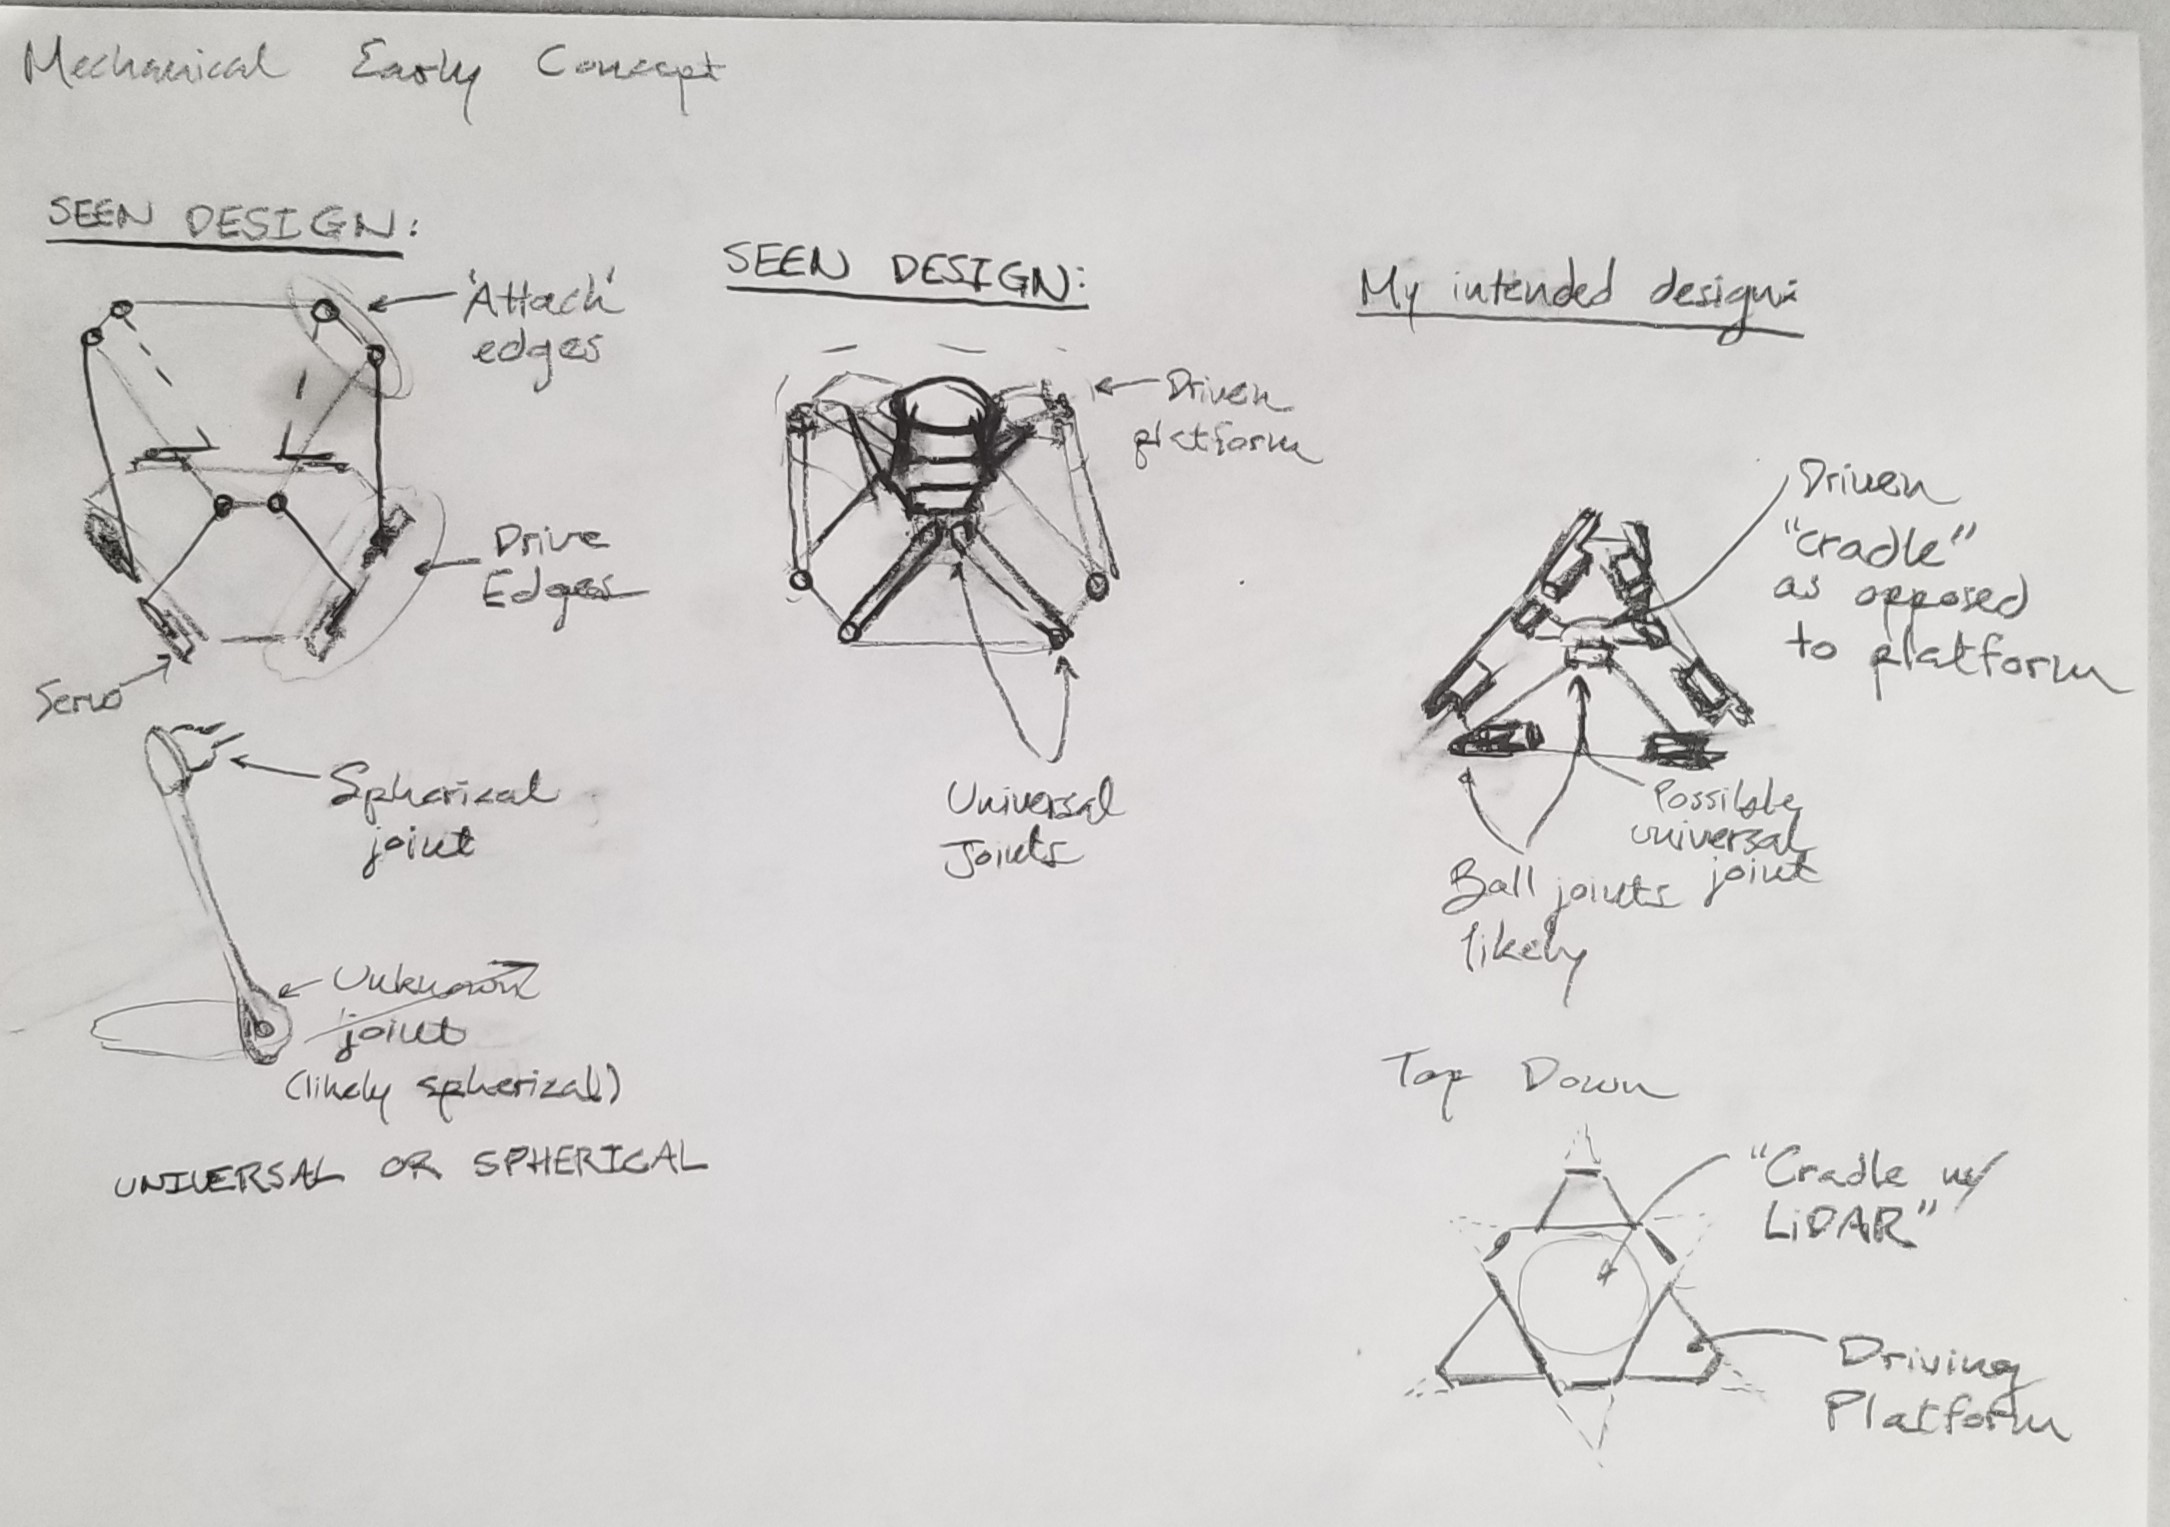
\includegraphics[scale=0.2]{early_mechanical}
			\caption{Mechanical sketches seen at the right}
			\label{basic_mechanical}
		\end{figure}
	
		The first version of the eye will probably just be for practice controls and mechanical effectiveness. The first and final will share the same motors, joints, and most mounting; however, the final will include additional mounting for fixture to the rover, improved linkages, and additional components to make the whole assembly water/rubble resistant. 
		
	\subsection{4/6/23}
		\subsubsection{Summary}
		Continued research into the design of the Stewart platform. Notes on many of the design projects and research papers were completed in the 'Scratch Notes' document found in the drive. Perhaps in the future some notes summarizing the math and theory behind Stewart platforms can be written.
	
	\subsection{4/7/23}
		\subsubsection{Summary}
		Continued research, like yesterday. Some part selection and purchasing based on my current knowledge. Didn't purchase ball joint linkages, but instead came up with a method of grabbing the 3D file desired from McMaster-Carr and printing; see an explanation below.
		
		\subsubsection{Roadblock: Horrible Prices...}
		In the design of the Stewart platform some threaded ball joint linkages were needed. Note that ball joint linkages and ball joints are different in that the former has a linkage built into the ball of the joint. When I tried to purchase these online I saw prices of \textbf{\$ 18.00 each}... and I need 12 of these minimum. Obviously this won't do, and plastic hobby ones found for resale on Ebay appear incredibly sketchy.
		
		Instead, I pick the ball joint linkage size I desire from McMaster-Carr, then press `download 3D model', (make sure it's set to download the STEP file). From there I can model with the STEP in Fusion360, or use an online, free converted to convert to STL, then print it. For things like ball joint linkages I strongly encourage you to use a resin printer, since it can print high resolution and threads pretty well.
		
		\begin{figure} [h]
			\centering
			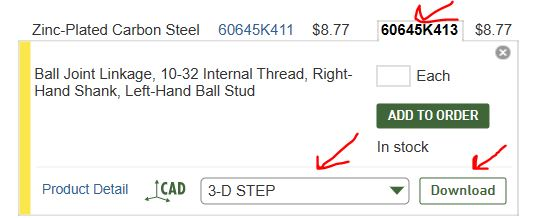
\includegraphics[scale=0.75]{mcmaster_models}
			\caption{Selecting a part, then file type, then download}
			\label{getting_models}
		\end{figure}
		
		When modeling with STEP files in Fusion360, it's advised to make slight modifications and redesigns for the purpose of 3D printing. Make sure to save both a Fusion360 part file and an STL version. If I do this with the ball joint linkages I'll detail and snapshot how I edited them.
		
	\subsection{4/9/23}
		\subsubsection{Summary}
		Continued research and mechanical modelling today. I found many parts through McMaster-Carr and GrabCAD so I didn't have to model them myself. The entire first iteration was modelled. Custom ball joints and servo horns were created.
		
		Models were output in the discord server to be printed; ball joints and horns on the resin printer, major jig on the FDM printer. Future developments in the 'sleekness' of the LiDAR housing, the mounting of servos, and some tolerances (especially for wires) should be considered.
		
		\subsubsection{Roadblock: Tricky Design Parameters}
		In designing on paper I found myself running into lots of intricately related design parameters. The mount that holds the LiDAR must obviously be based on the LiDAR's major diameter; however, it must also roughly match, yet be smaller, than the `circular' array of servos; by which I mean the circle that circumscribes all points on the triangle the servo's are placed on. The reason is to not occupy a large default angle, giving us more room for motion. Assuming this to be the case then the servos have to be arranged first, the horns have to be placed, and the linkages placed on the horns. From there a circle slightly smaller than the servos' circle is created some appreciable distance away from the face of the servo housing; this circle defines the location of the attach points for the upper platform. The rest of the upper platform is built around this.
		
		The design involves plenty of reference and construction geometry. The base servo circle was referenced from \textbf{another} circle which transcribed all 6 vertices of the unequal hexagon, whos larger side length was based on 2 servo lengths, 1 gap length, and 2 constants for a total length of a kind number. You can see this hexagonal shape in the very first sketch created in the assembly file. From there some `wings' were extruded to support the servos. From platform center to furthest vertex a radius of roughly 7'' extends. A smaller, driven cradle was then created slightly smaller in radius of roughly 6'', placed such that the face of the LiDAR sits 5'' above the baseplate. Note that this LiDAR distance isn't set in stone, the linkages will dictate the final location. The details of design are self explanitory through the Fusion360 design history.

\clearpage

		The final product can be seen in figure \ref{3D_view} with the LiDAR, servos, and ball joint linkages visualized; though the linkages connecting the two platforms are not visible.
		
		\begin{figure} [!h]
			\centering
			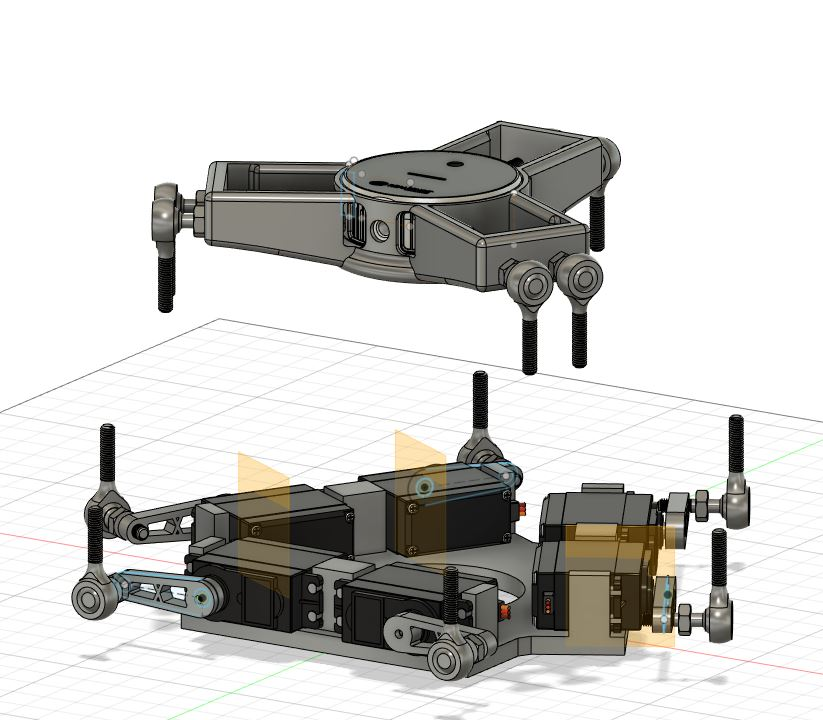
\includegraphics[scale=0.35]{complete_assembly}
			\caption{A 3D view of the completed first iteration}
			\label{3D_view}
		\end{figure}

		If you look down from the top (as seen in figure \ref{top_down}) you might be able to pick out the two triangles fashioned to the Star of David. Note that the closest, adjacent ball joint linkages will be connected.
		
		\begin{figure} [!h]
			\centering
			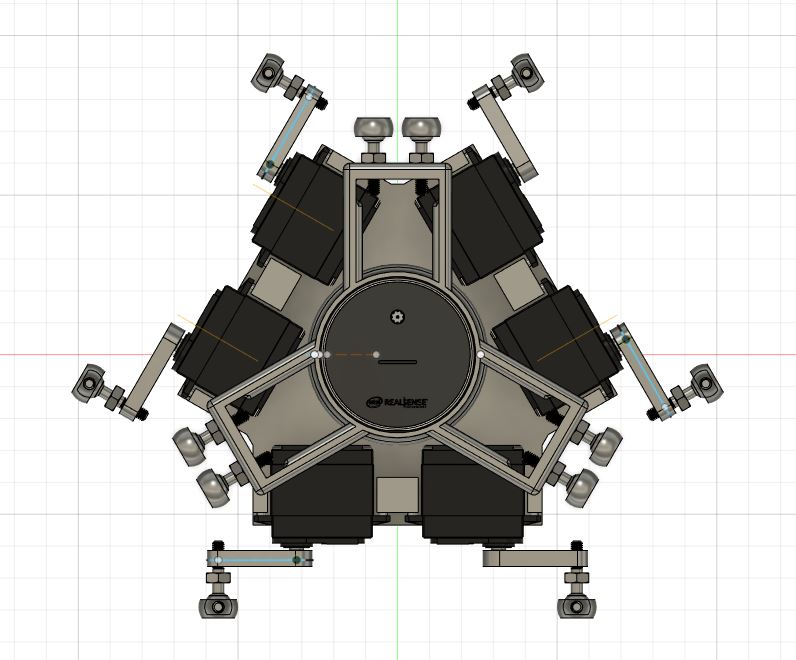
\includegraphics[scale=0.4]{assembly_top_down}
			\caption{Selecting a part, then file type, then download}
			\label{top_down}
		\end{figure}
		
		\subsubsection{Roadblock: Unfit Ball Joint Linkages}
		The ball joint linkages were presumably manufactured to just be balls in an close fit socket, rotating on their contact. This wouldn't work for 3D printing (as the slicer would bring the ball and socket together), so modifications had to be made. The socket was designed to actually house a ball that has a printable gap. I also made sure to shrink the ball neck as to give more motion. Finally, the bottoms were extended and lined up to permit easy printing; only the threads of the stud should need support. Visuals can be seen in  figure \ref{ball_joint}.
		
		\begin{figure*}[h]
			\centering
			\begin{subfigure}[h]{0.34\textwidth}
				\centering
				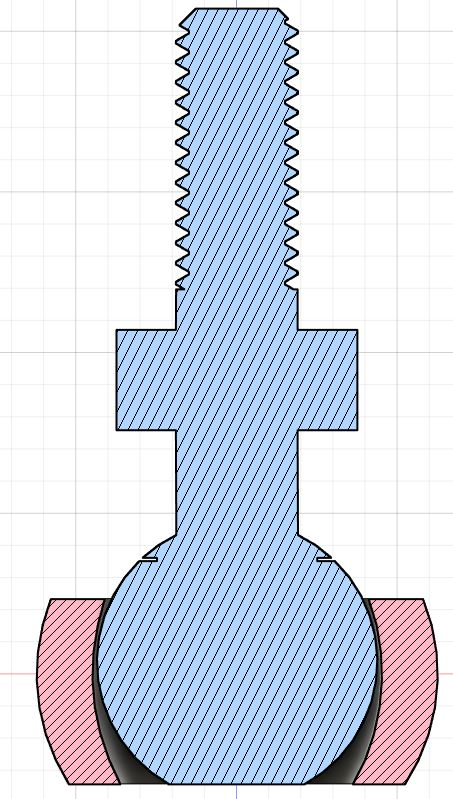
\includegraphics[width=\textwidth]{section_ball_joint}
			\end{subfigure}
			\hfill
			\begin{subfigure}[h]{0.65\textwidth}
				\centering
				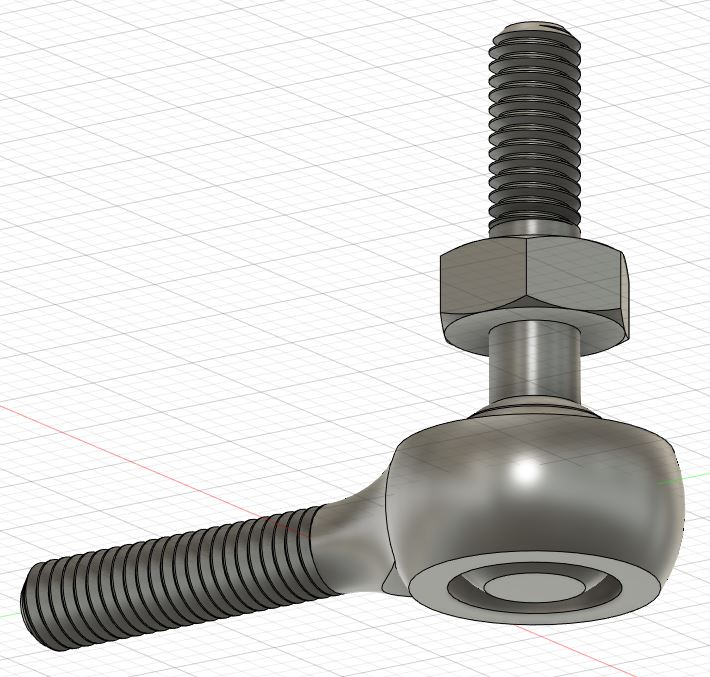
\includegraphics[width=\textwidth]{ball_joint}
			\end{subfigure}
			\centering
			\caption{Section of the ball joint showing no interference, next to its 3D model}
			\label{ball_joint}
		\end{figure*}
		
	\subsection{References/Resources}
	\begin{itemize}
		\item A great example which includes a lot of mention of kinematics is seen \href{https://ntrs.nasa.gov/api/citations/19910007810/downloads/19910007810.pdf}{here}
		\item What might be called a treatise on Stewart platforms is found \href{https://www.ri.cmu.edu/pub_files/pub4/fong_terrence_w_1990_1/fong_terrence_w_1990_1.pdf}{here}
		\item An instructables on making a ghetto Stewart platform with Servos \href{https://www.instructables.com/Stewart-Platform/}{here}
		\item All robotic devices need kinematics models to work; \href{https://www.xarg.org/paper/inverse-kinematics-of-a-stewart-platform/}{this article} provides a kinematic model for Stewart platforms powered by rotary means (ie servo)
		\item Another good design example found \href{https://iopscience.iop.org/article/10.1088/1757-899X/563/5/052059/pdf}{here}
		\item Though it uses linear actuators, has some good examples of tests that might be performed on Stewart platforms \href{https://www.ncbi.nlm.nih.gov/pmc/articles/PMC6513003/}{here}
		\item Another good \href{https://core.ac.uk/download/pdf/322824733.pdf}{design example}
		\item A good \href{https://www.instructables.com/Six-Axis-Platform-Using-Linear-Actuators-Stewart-P/}{instructables}; however, this one uses linear actuators
		\item A good \href{https://www.ohio.edu/mechanical-faculty/williams/html/PDF/IndRob02.pdf}{design example} with potentially useful testing procedures
		\item A \href{https://www.mdpi.com/2218-6581/7/2/30}{lovely design} that looks nice and has a nice circular platform
		\item No tutorial, just great \href{https://www.youtube.com/watch?v=kscvCQTtVvw&t=0s}{inspiration}
		\item \textit{Parallel Robots} by J.P. Merlet
		\item \textit{Introduction to Robotics: Analysis, Control, Applications} by Saeed Niku
	\end{itemize}
	
	
\newpage	
	
\section{Electrical Design}
	\subsection{4/5/23}
		\subsubsection{Summary}
		Today some work was done in the way of planning the electrical; however, it relies all on existing knowledge of electronics. I may do more research in the future to ensure the the electrical is robust and end up changing the plans. Currently a solderable GikFun board will be used to provide all power and convey signal. Additionally, an Arduino Mega will be used for direct control of servos, but will recieve its instructions from the Nano. 
		
		Pins 2-7 on the Mega will convey logic through the GikFun board to the 6 movement servos, while pipns 10-11 will convey logic to the 'eyelids' of the protective housing. The GikFun will have a 5V barell jack that will recieve power from the PCB PDS of the rover. The Mega will recieve power from the GikFun, also a barell jack. The Mega will also be connected to the Nano via a standard USB printer cable. The Mega and Nano will communicate through ROS. An image below of the rough schematic can be seen.
		
		\begin{figure} [h]
			\centering
			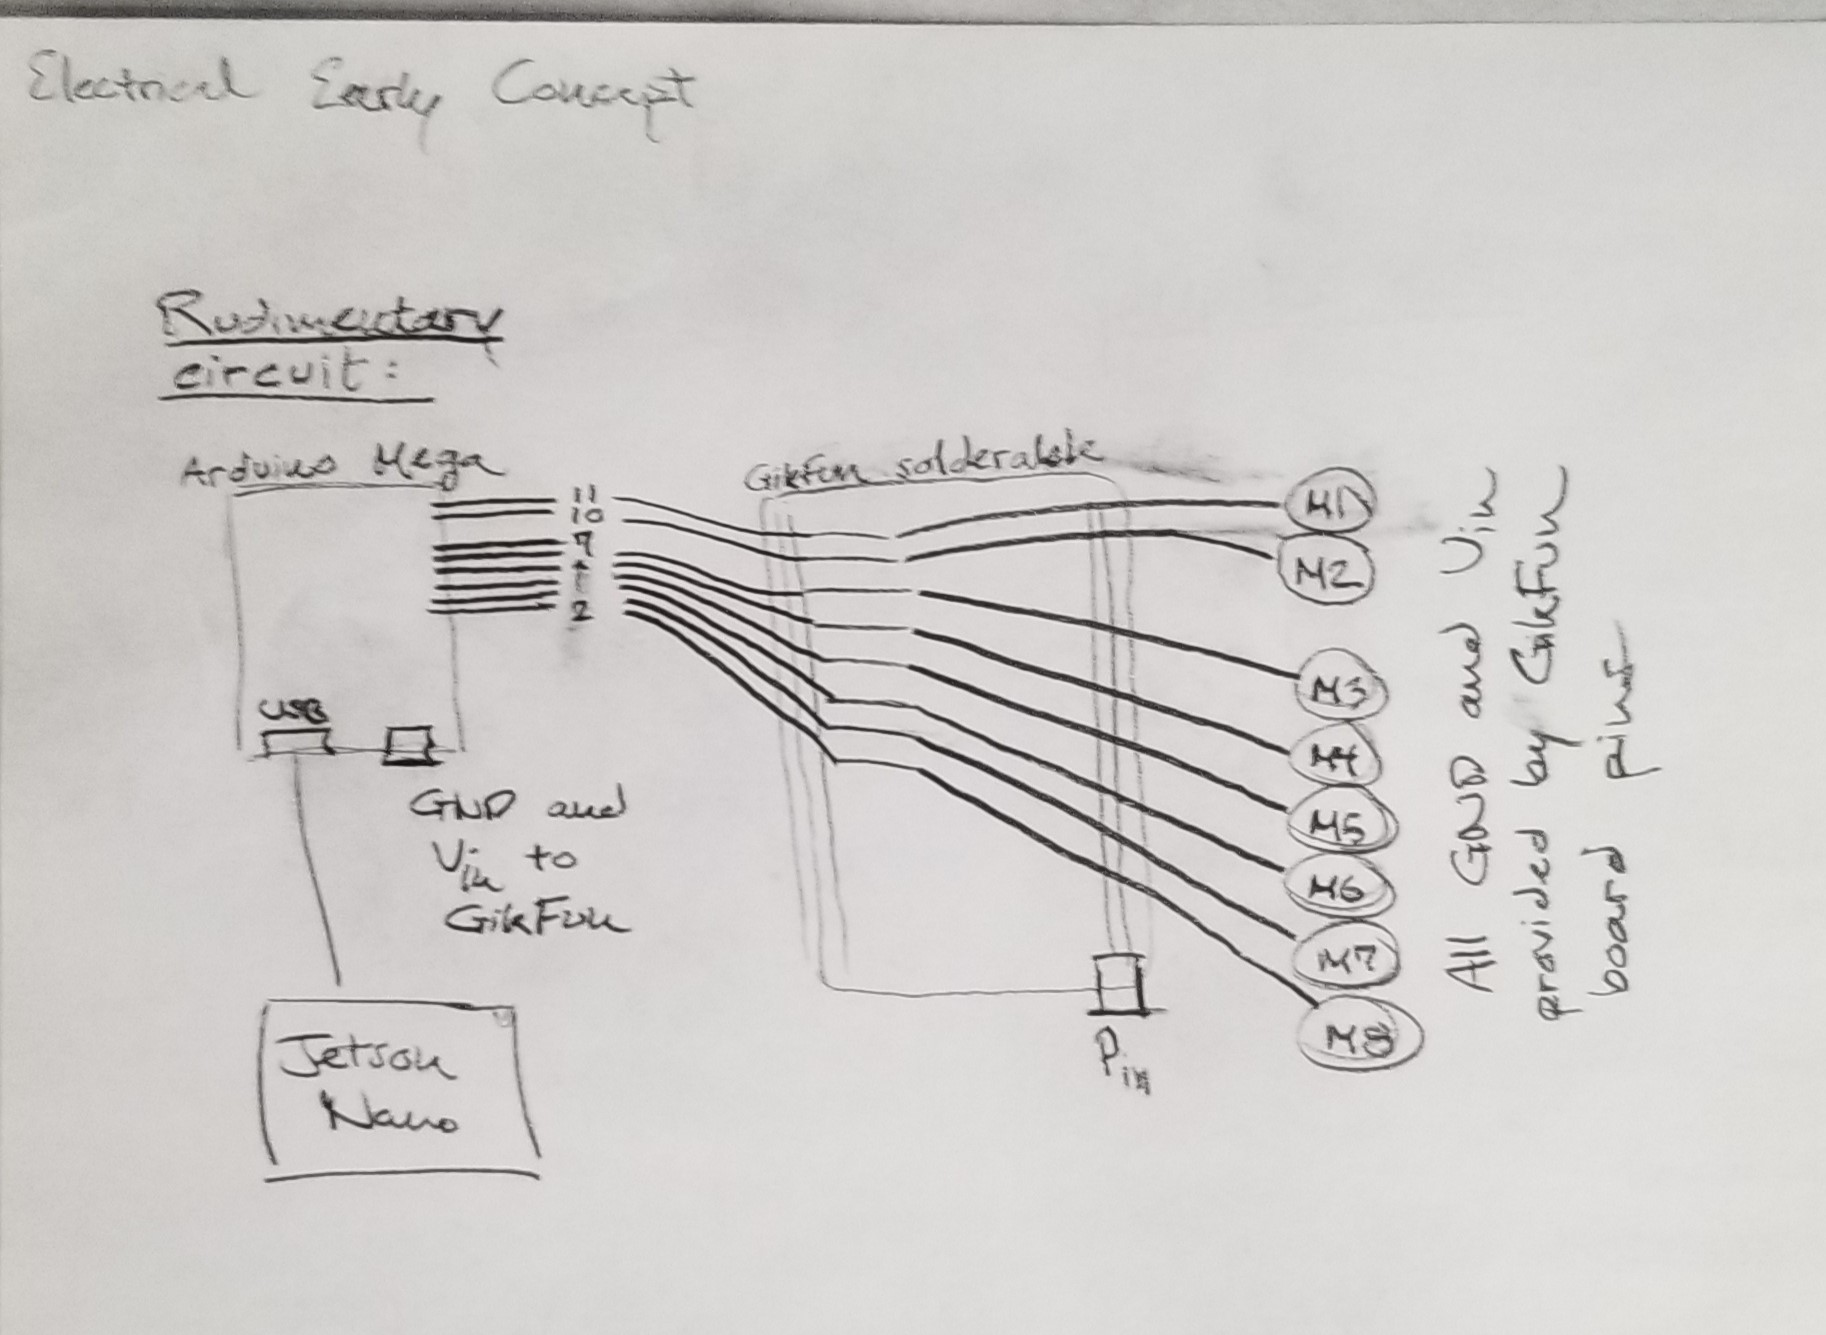
\includegraphics[scale=0.2]{early_electrical}
			\caption{Rudimentary electrical sketches}
			\label{basic_electrical}
		\end{figure}
		
	\subsection{4/7/23}
		\subsubsection{Summary}
		Some thought worth noting was put into the electrical. A 3D model of the complete circuit will be completed, and then a housing created. The printable housing will act as a sort of 'guide' for soldering components. 
		
		Because of it's superior clock speed, RAM, and electronics, we'll be opting to use the Arduino Due over the Mega. The Due has the exact same footprint as the Mega so nothing will change in the schematics.
	\subsection{References/Resources}

\end{document}